\chapter{System Setup}
The end system has two arrays, each with three microphones mounted on the vertices of a $20$ cm equilateral triangle. A micro-controller is attached to one of the vertices. Fig~\ref{fig:setup_array} shows a picture of the array setup. The micro-controller used in this project is \emph{teensy 3.1}, which has $64$k RAM memory and the ADC is capable of sampling at $500$kHz~\cite{tdoa:micloc, sys:teensy}. In this project, the micro-controller collects microphone data on all three channels for $12$ milliseconds and then sends the recorded data to a computer through the USB port for localization. 

\begin{figure}[]
  \centering
  \begin{subfigure}[]{.23\textwidth}
    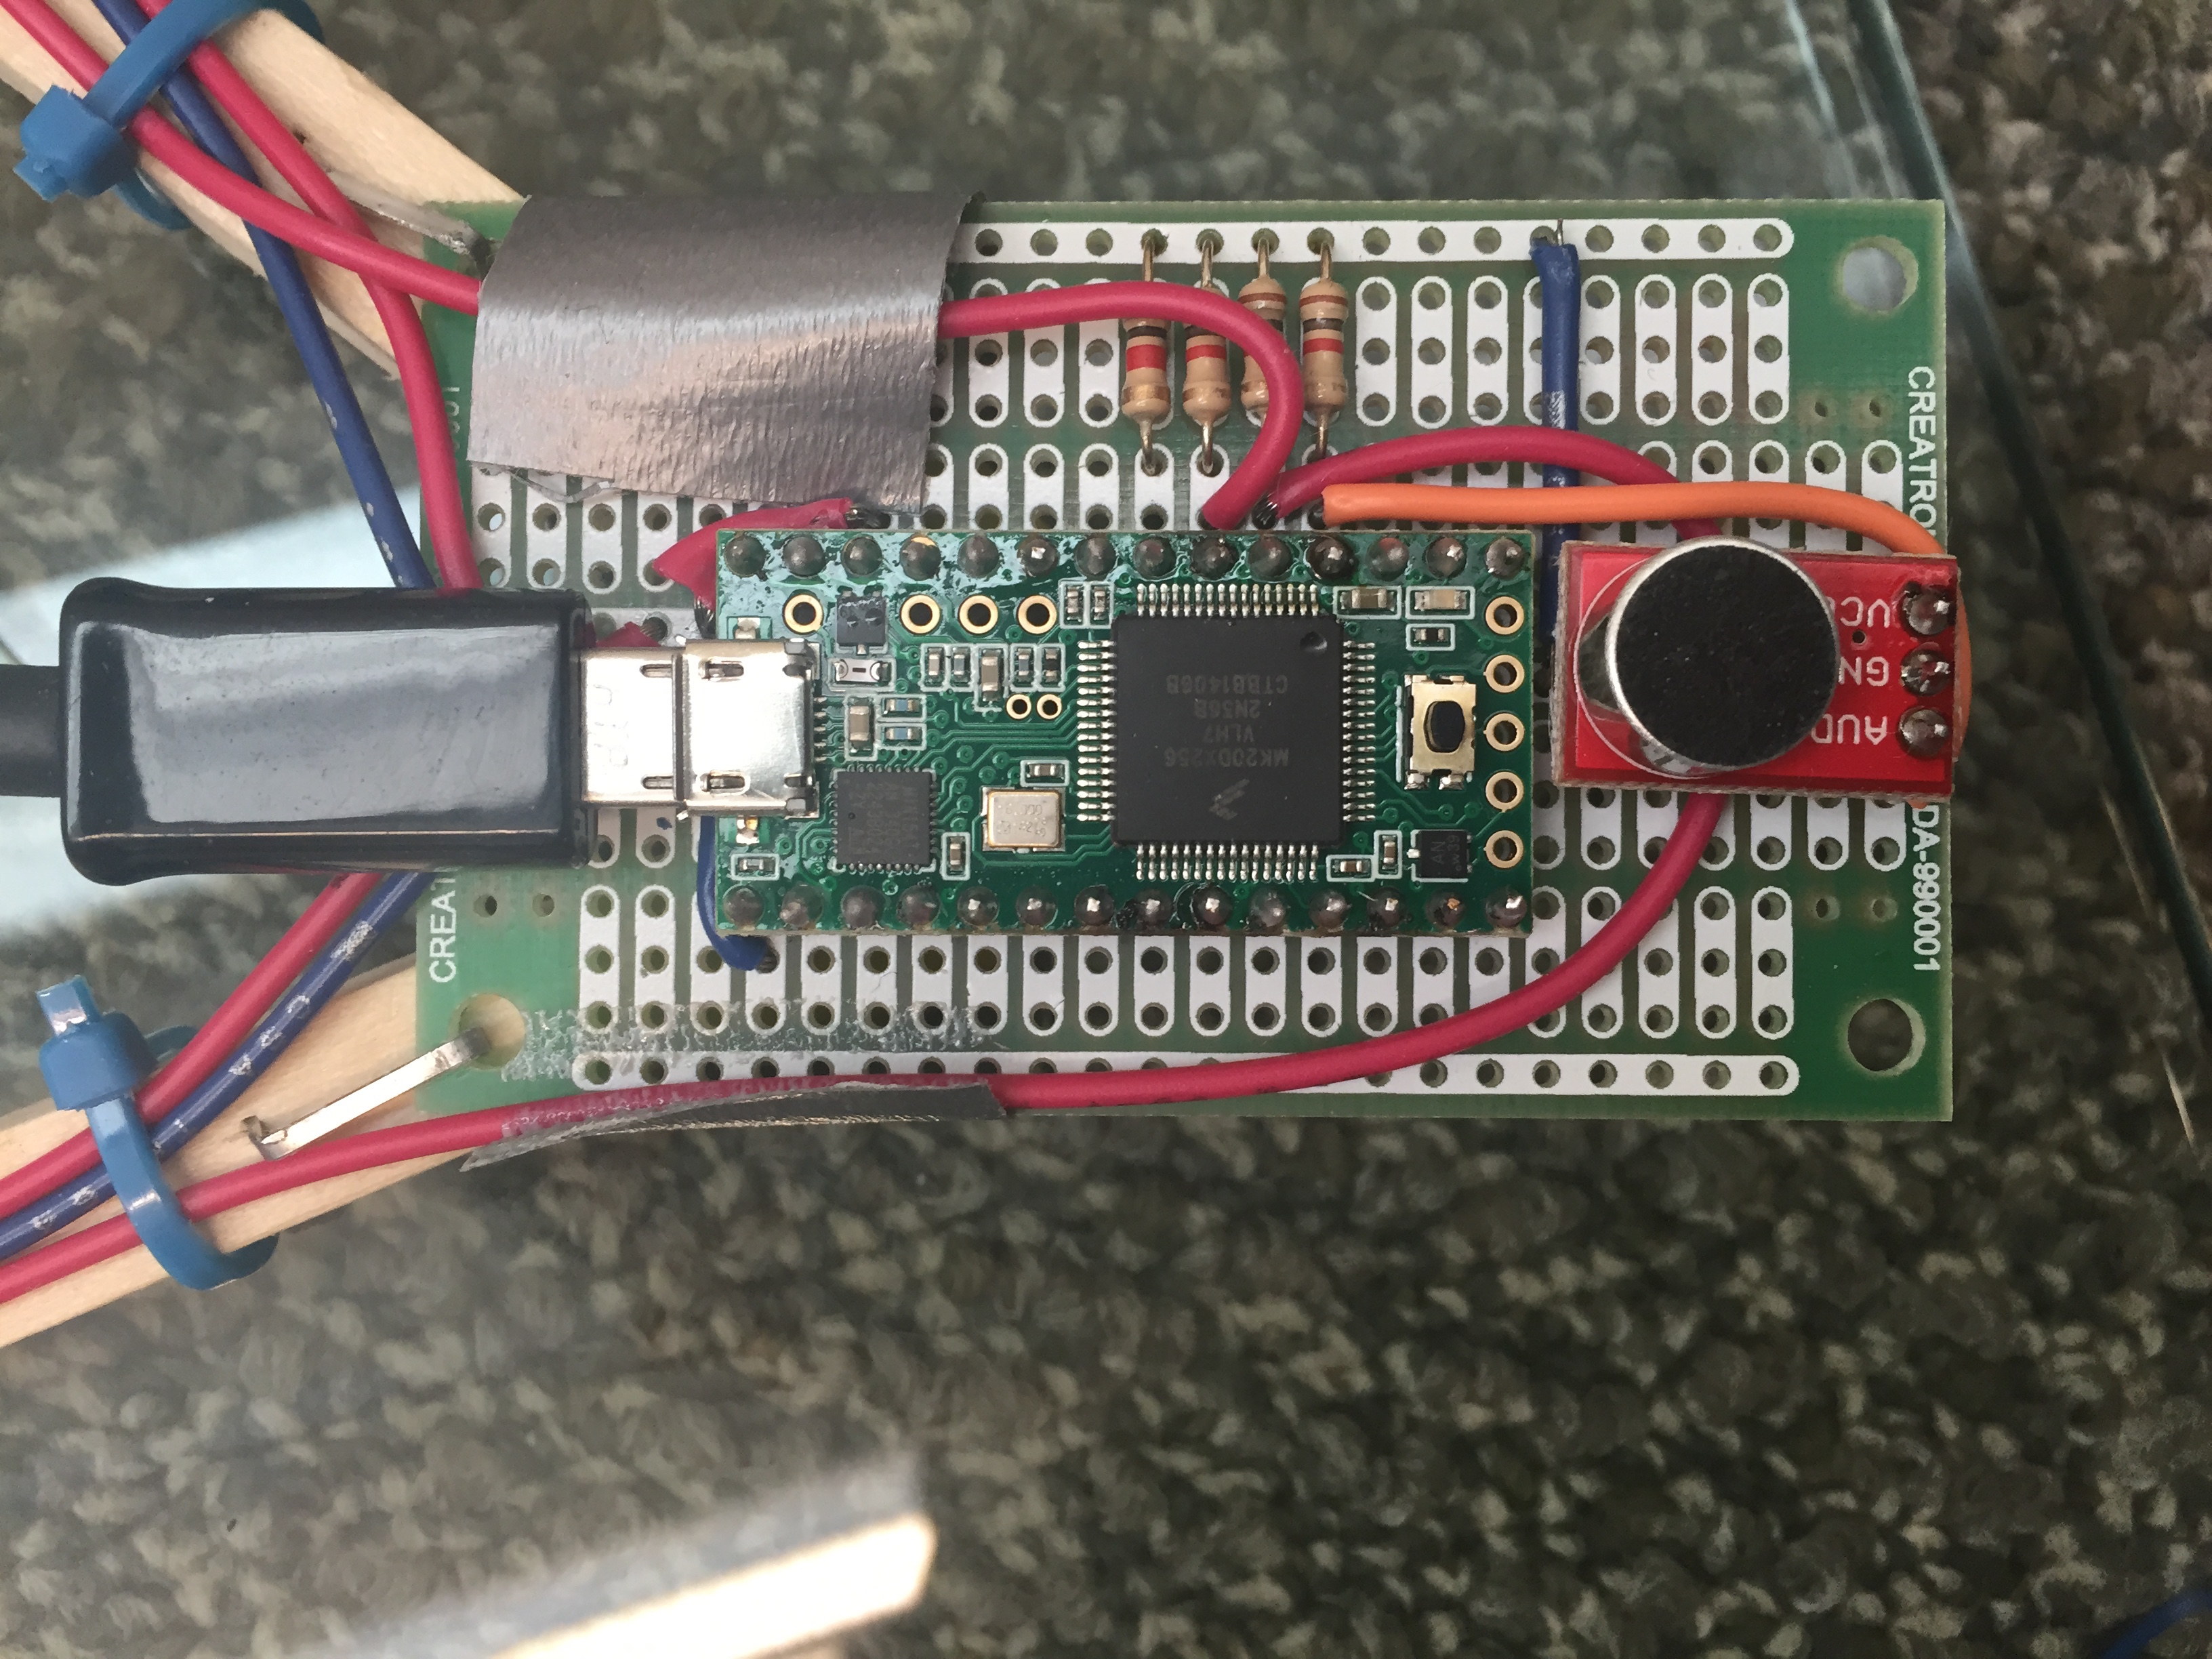
\includegraphics[width=\textwidth]{array_close.JPG}
    \caption{micro-controller}
  \end{subfigure}
  \begin{subfigure}[]{.23\textwidth}
    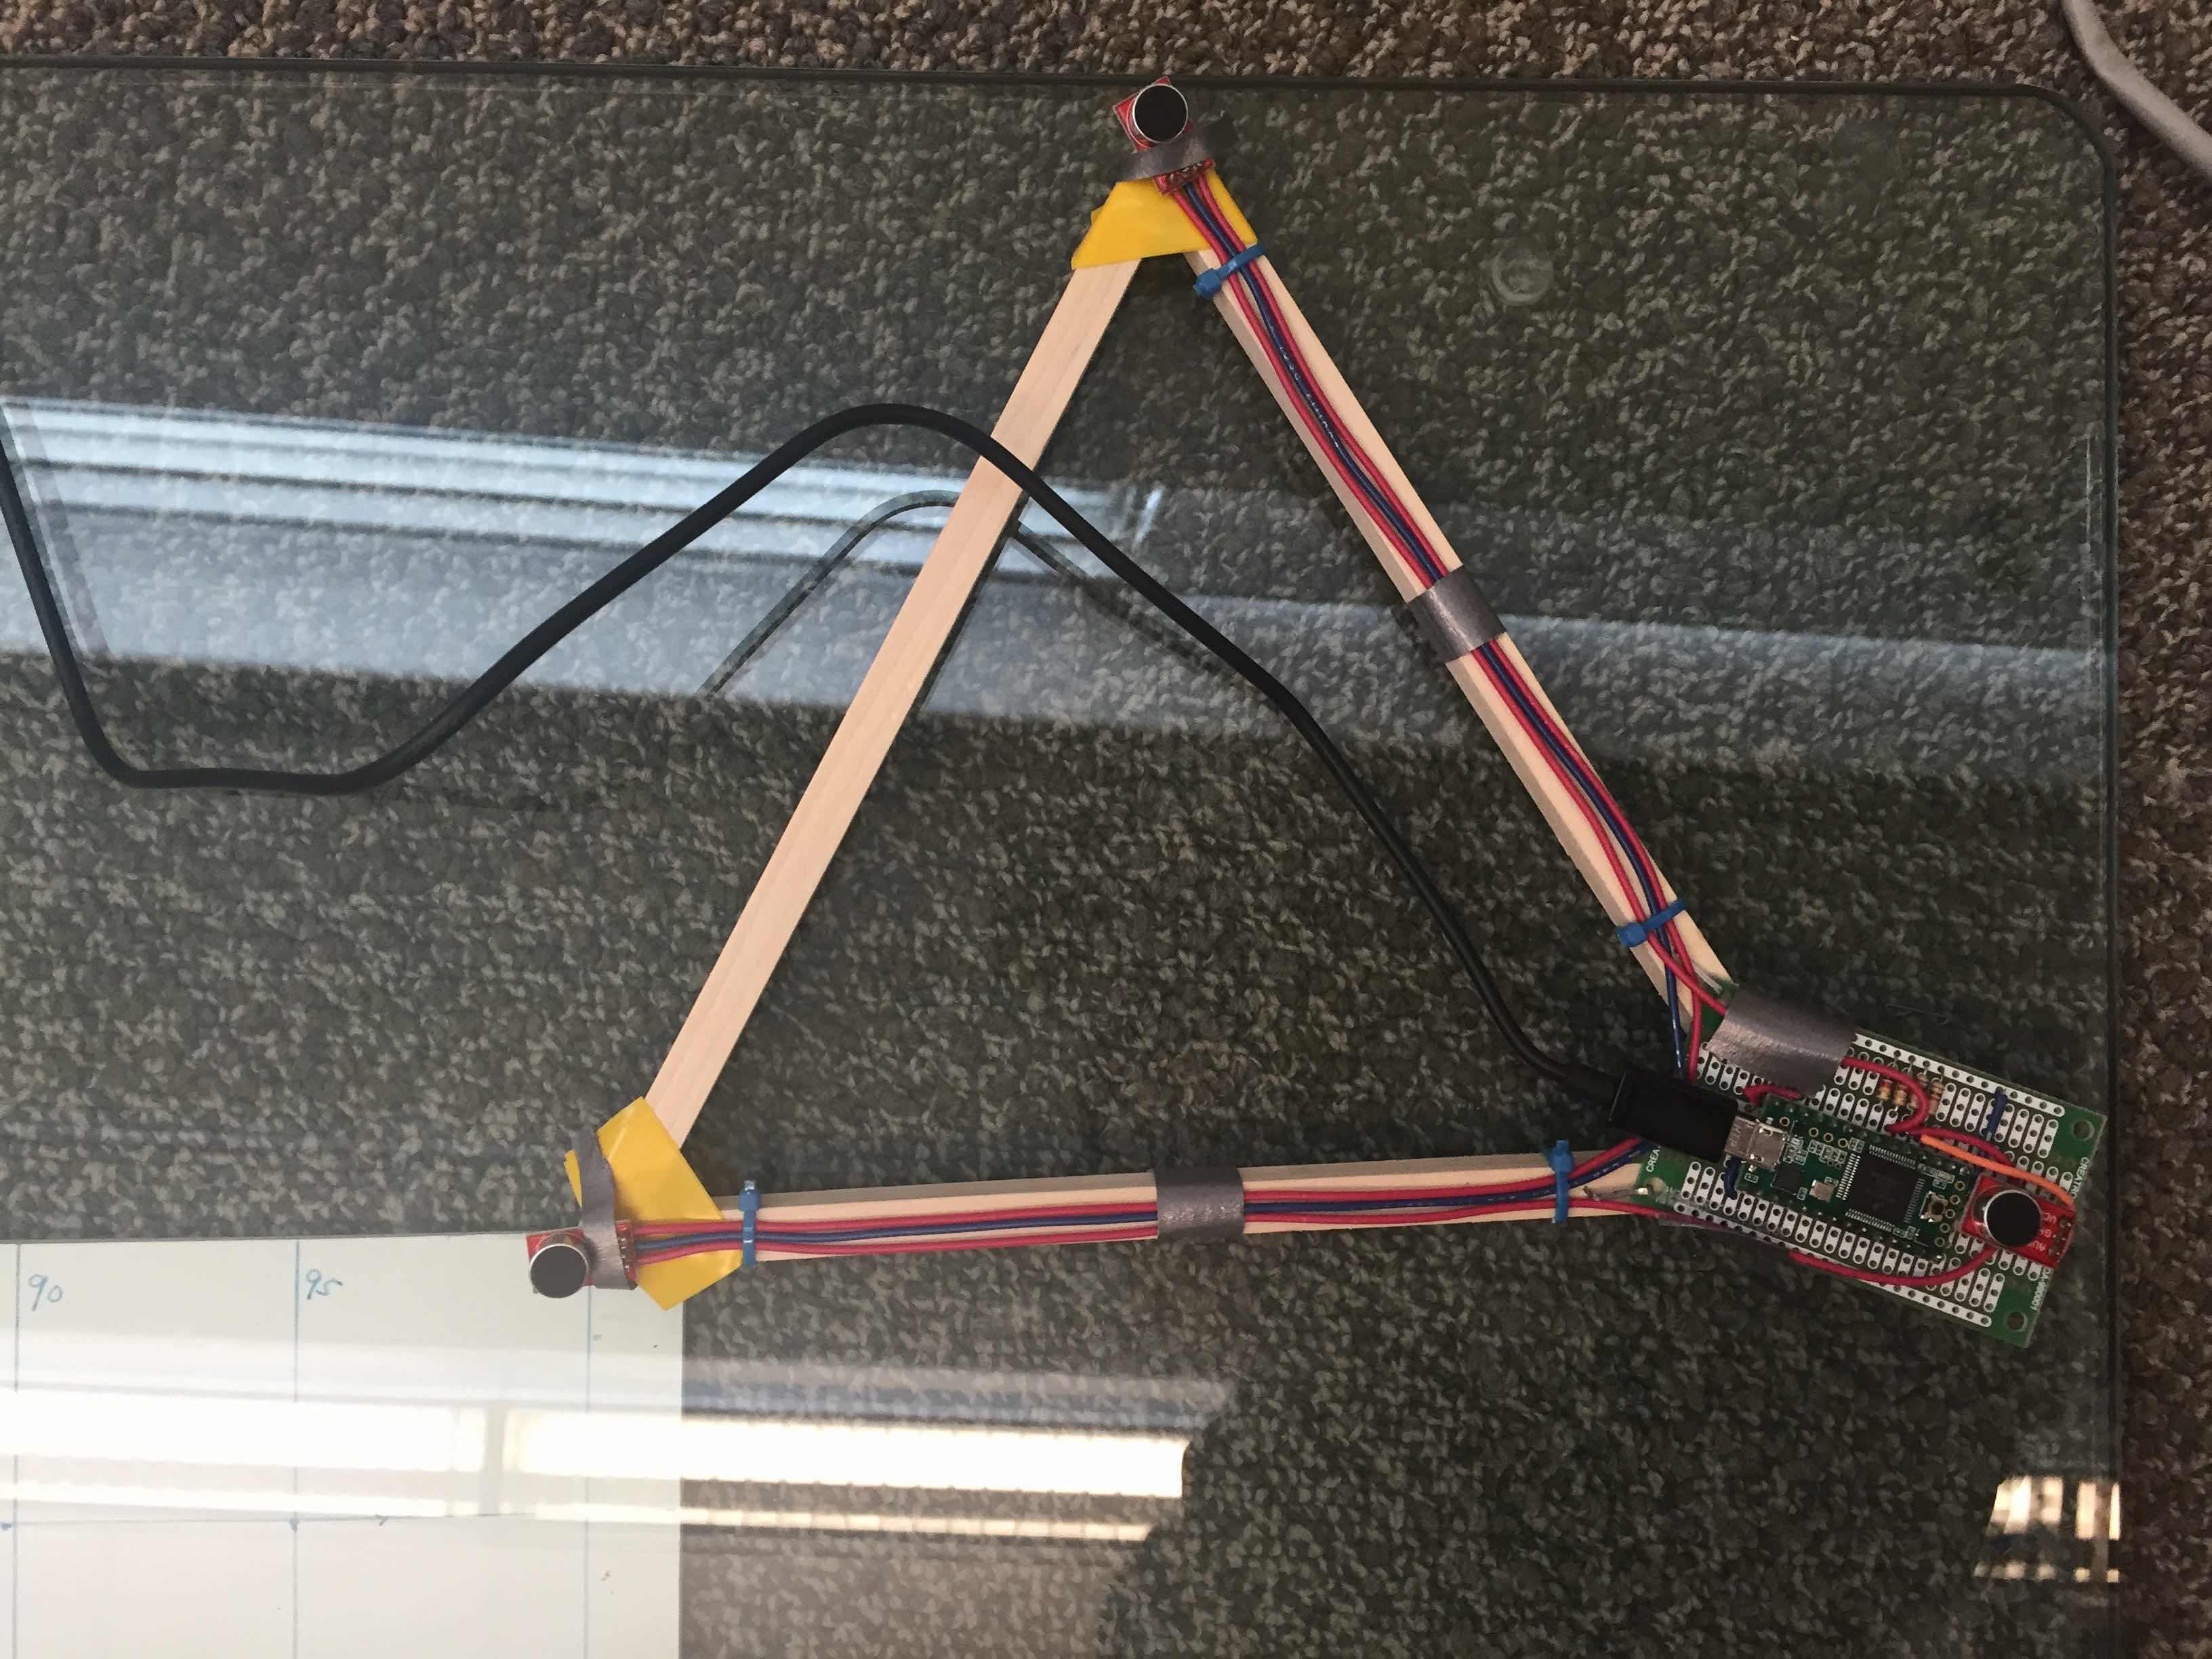
\includegraphics[width=\textwidth]{array.JPG}
    \caption{array}
  \end{subfigure}
  \begin{subfigure}[]{.23\textwidth}
    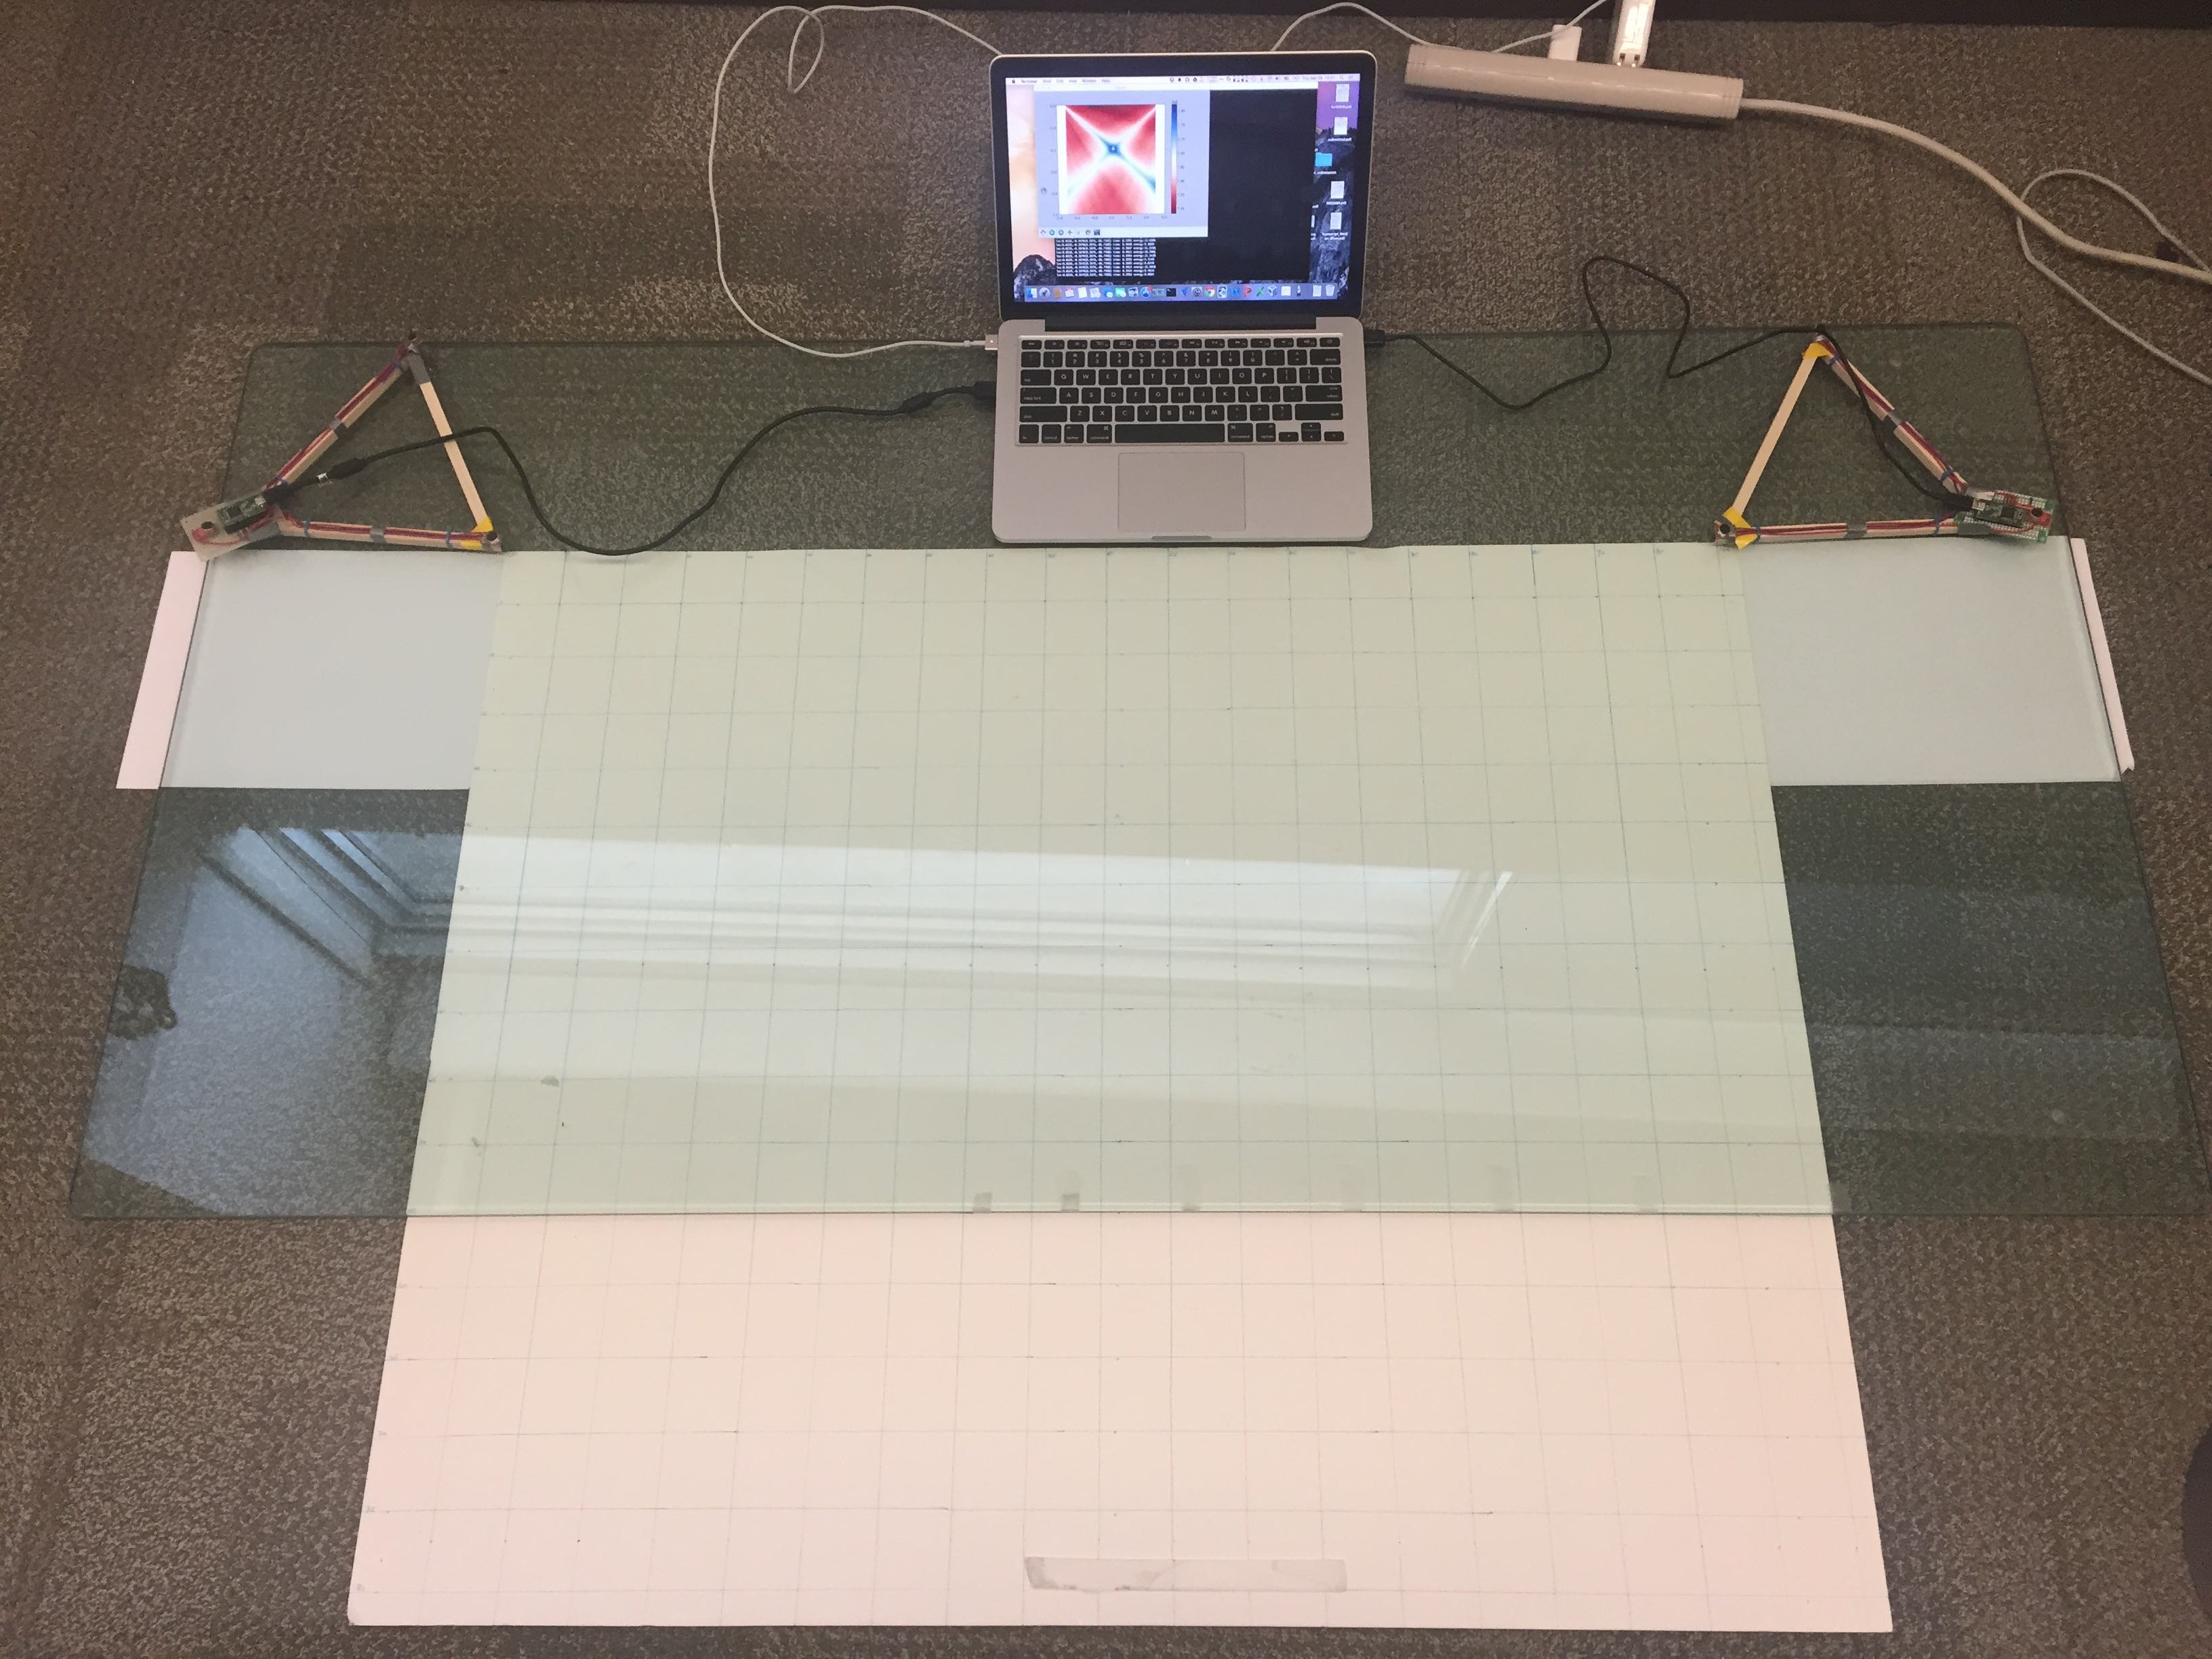
\includegraphics[width=\textwidth]{setup_2.JPG}
    \caption{two arrays}
  \end{subfigure}
  \caption{Localization system setup}
  \label{fig:setup_array}
\end{figure}

To handle the uncertainty in TDOA estimation, instead of using point estimate that maximizes equation~\ref{eq:gcc}, we take the cross-correlation output(equation~\ref{eq:gcc2}) as a measure of the likelihood of different arrival time differences. For each microphone array, we build a heatmap for the region. The intensity at each point represents the likelihood of it being the source. For each point on the grid, the theoretical TDOA to each microphone pair can be precomputed. Then the heatmap can be generated by going through points on the grid and performing a lookup using equation~\ref{eq:gcc2}. With three microphones $m_1,m_2,$ and $m_3$, there are three microphone pairs: $m_1m_2,m_1m_3,$ and $m_2m_3$. The theoretical TDOA from each location $(x,y)$ to each microphone pair is precomputed and stored in $D_{m_1,m_2}(x,y)$, $D_{m_1,m_3}(x,y)$, and $D_{m_2,m_3}(x,y)$. Then the likelihood map $L(x,y)$ can be built by superposing the likelihood from each microphone pair:
\begin{eqnarray*}
L(x,y) &=& R_{m_1,m_2}(D_{m_1,m_2}(x,y)) + R_{m_1,m_3}(D_{m_1,m_3}(x,y)) \\
 & & +R_{m_2,m_3}(D_{m_2,m_3}(x,y)) 
\end{eqnarray*}
,where $R_{m_1,m_2}(\tau)$,$R_{m_1,m_3}(\tau)$, and $R_{m_2,m_3}(\tau)$ denote GCC output from microphone pairs $m_1m_2,m_1m_3,$ and $m_2m_3$.

Likelihood maps from two arrays can be combined into the final likelihood map:
\begin{equation}\label{eq:combine_l}
L(x,y) = L_1(x,y) L_2(x,y)
\end{equation}
, where $L_1(x,y)$ and $L_2(x,y)$ represent the likelihood map from array $1$ and array $2$.

\begin{figure}[]
  \centering
  \begin{subfigure}[]{.23\textwidth}
    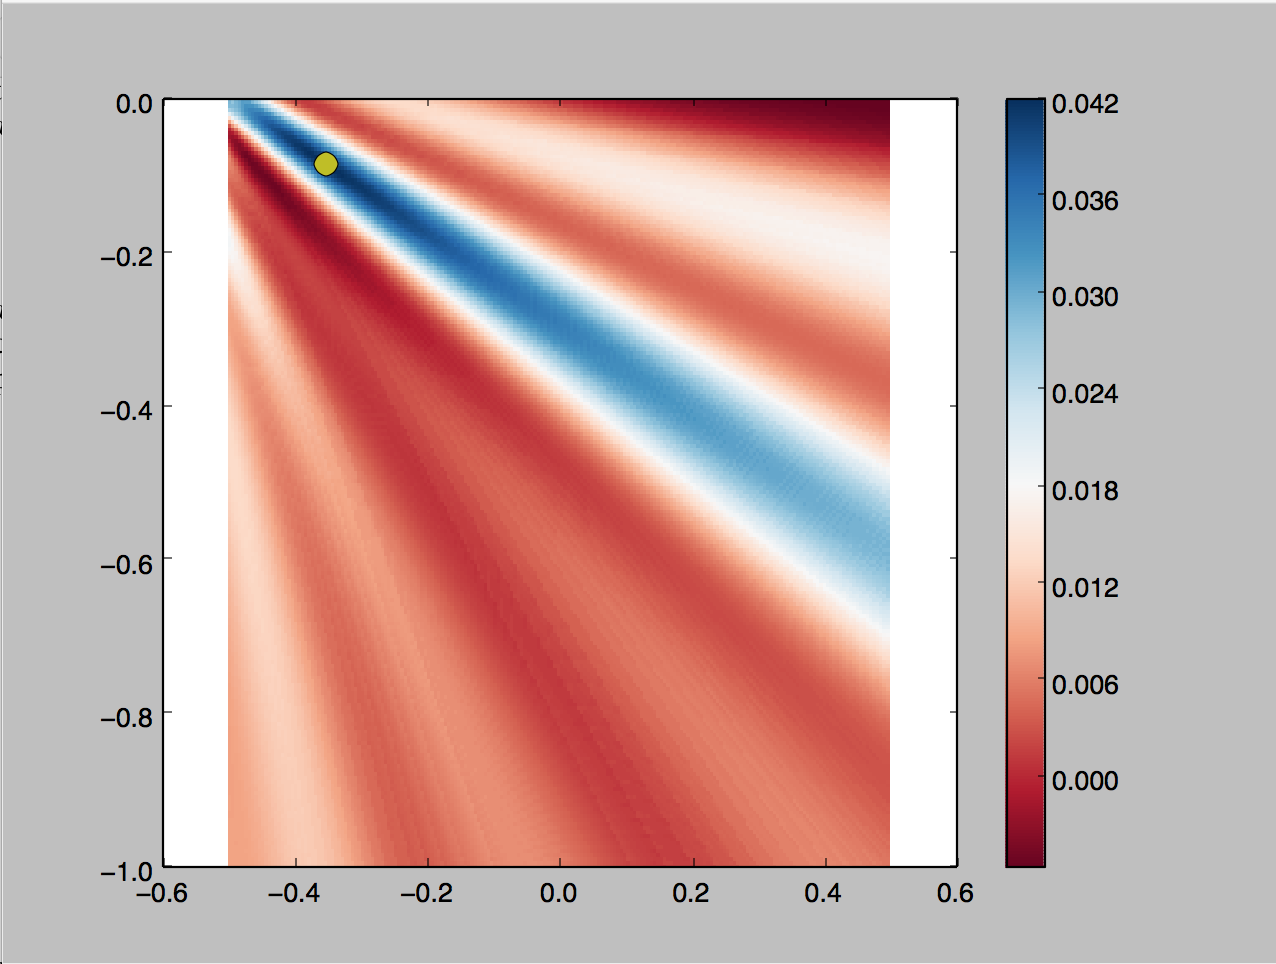
\includegraphics[width=\textwidth]{left.png}
    \caption{localization with only array 1}
    \label{fig:liklihood1}
  \end{subfigure}
  \begin{subfigure}[]{.23\textwidth}
    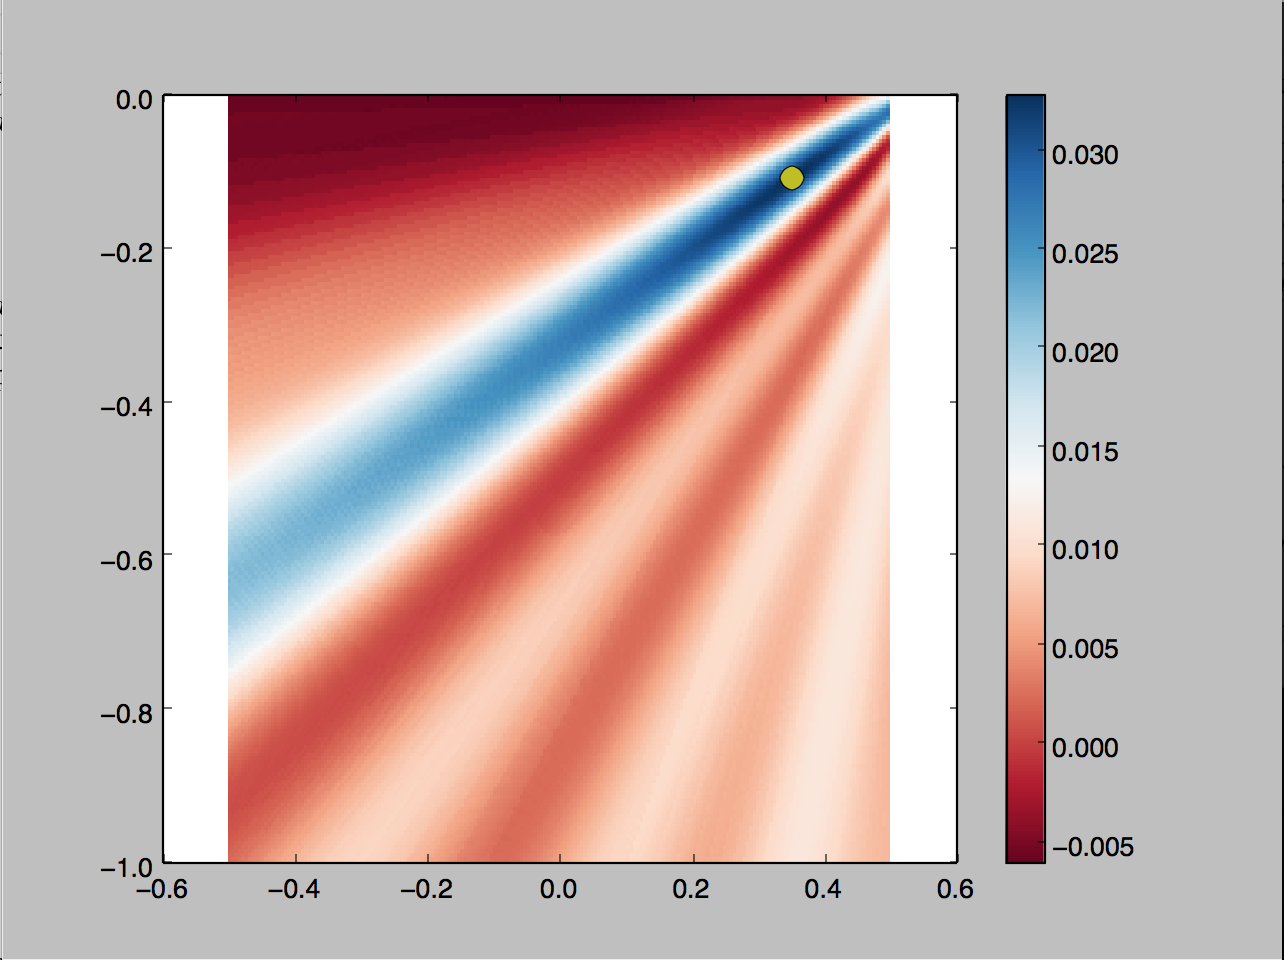
\includegraphics[width=\textwidth]{right.png}
    \caption{localization with only array 2}
    \label{fig:liklihood2}
  \end{subfigure}
  \begin{subfigure}[]{.23\textwidth}
    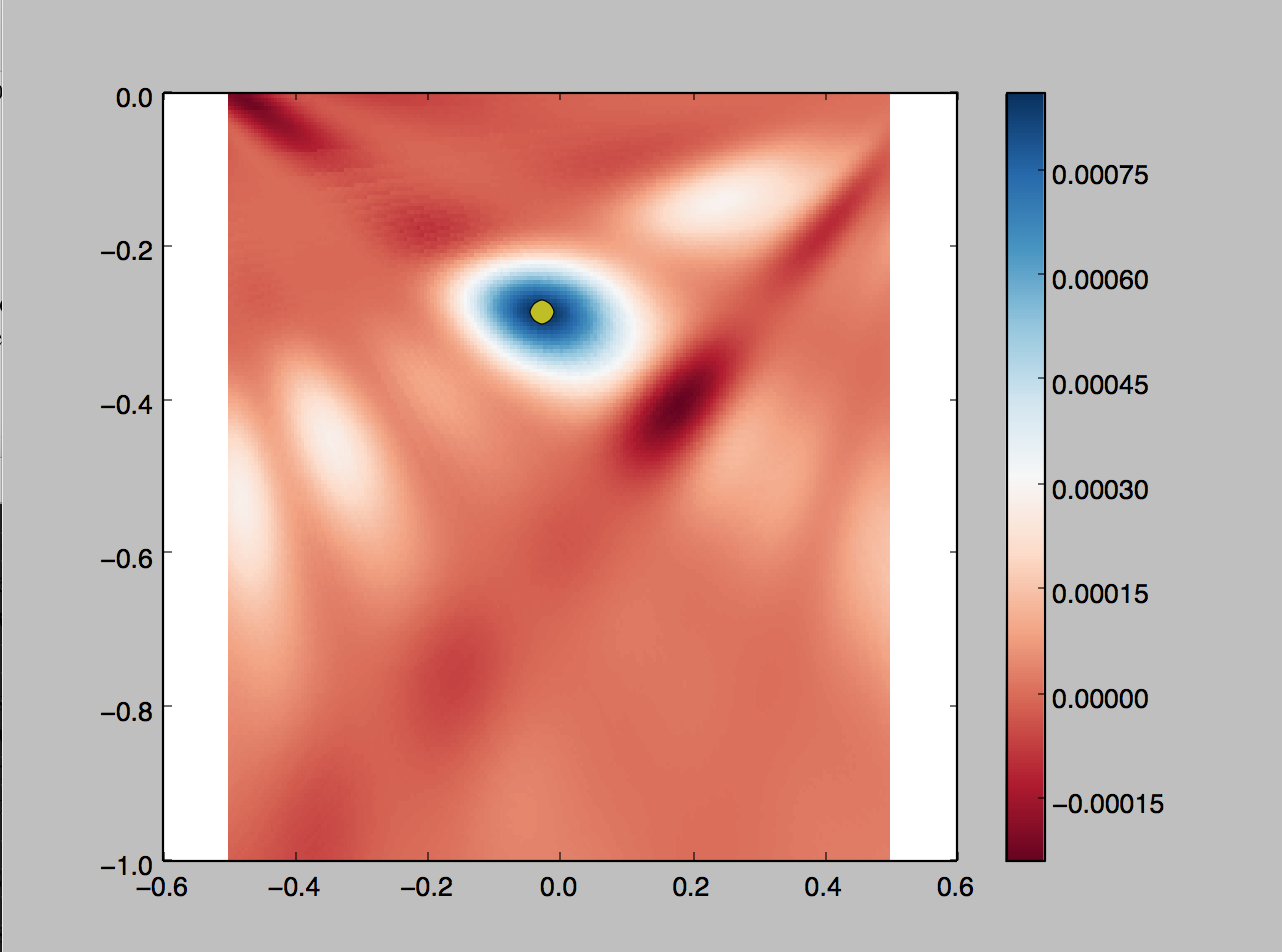
\includegraphics[width=\textwidth]{combined.png}
    \caption{localization with both arrays}
    \label{fig:liklihood3}
  \end{subfigure}
  \caption{Likelihood maps for localization. The source is placed at $(0.0,-0.3)$ m}
  \label{fig:liklihood}
\end{figure}

To see the effect of accuracy improvement using multiple arrays, fig~\ref{fig:liklihood} shows a real life localization where the source is placed at $(0$ cm$,-30$ cm$)$. It shows the individual likelihood map from each array and also the combined likelihood map according to equation~\ref{eq:combine_l}. Individual arrays give accurate angle estimate, but have high uncertainty in distance estimate. The combined likelihood map demonstrated that by merging estimates from two arrays the system is able to perform more accurate localization. 

From a timing point of view, the micro-controller spends $12$ milliseconds on sampling the microphone data before sending it to a computer for processing. Sending the data through the USB port takes another $15$ milliseconds, and processing on the computer takes around $50$ milliseconds. Therefore, the total time lag between sound source and localization is around $80$ milliseconds.
